{\bf Задача была переформирована на интерактивную парадигму. }

Рассмотрим игру для двух игроков. Игрокам дан прямоугольник размером $x \times y$ (где $x$ и $y$~--- положительные целые числа). 
Игроки ходят по очереди. Ход состоит в разделении прямоугольника на два прямоугольника одним горизонтальным или вертикальным разрезом. 
Полученные прямоугольники должны иметь положительные целочисленные размеры.

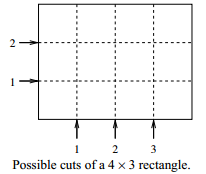
\includegraphics{rectangle.png}

Возможные разрезы прямоугольника размером $4 \times 3$.

После каждого разреза прямоугольник с меньшей площадью убирается, а оставшийся передается другому игроку. 
Если прямоугольник разделен на две равные части, то убирается одна из них.
Игрок, который получает прямоугольник размером $1 \times 1$, проигрывает, так как не может сделать следующий ход.

Ваша задача~--- написать программу, которая бы играла в игру с прямоугольниками и выигрывала. 
Начальные размеры прямоугольника~--- целые числа от $1$ до $100\,000\,000$. 
Как минимум один из размеров больше 1. 
